% Nishant D. Gurnani - Senior Thesis
% Main Latex File

% FORMATTED FOR THESIS BINDING
\documentclass[11.75pt,oneside]{amsart}
\usepackage[top=1in, left=1.5in, right=1in, bottom=1in]{geometry}

\usepackage{geometry}
\usepackage{amsmath,amssymb}
\usepackage{hyperref}
\geometry{letterpaper}

% For figures
\usepackage{graphicx} % more modern
\usepackage{subfigure} 
\usepackage{float}
\floatstyle{boxed}
\restylefloat{figure}

% For ceiling function
\usepackage{mathtools}
\DeclarePairedDelimiter{\ceil}{\lceil}{\rceil}


\newcommand{\id}{\mathrm{id}}
\newcommand{\K}{\mathrm{KL}}
\newcommand{\kl}{\mathrm{kl}}
\newcommand{\bp}{\boldsymbol{p}}
\renewcommand{\phi}{\varphi}
\renewcommand{\a}{\alpha}

\renewcommand{\P}{\mathbb{P}}
\newcommand{\E}{\mathbb{E}}
\newcommand{\N}{\mathbb{N}}
\newcommand{\R}{\mathbb{R}}
\newcommand{\Q}{\mathbb{Q}}
\newcommand{\KL}{\mathrm{KL}}
\newcommand{\LG}{\overline{\log}(d)}
\newcommand{\LGG}{\overline{\log}(M K)}
\newcommand{\ocP}{\overline{\mathcal{P}}}

\newcommand{\cO}{\mathcal{O}}
\newcommand{\cZ}{\mathcal{Z}}
\newcommand{\cA}{\mathcal{A}}
\newcommand{\cB}{\mathcal{B}}
\newcommand{\cN}{\mathcal{N}}
\newcommand{\cM}{\mathcal{M}}
\newcommand{\cF}{\mathcal{F}}
\newcommand{\cL}{\mathcal{L}}
\newcommand{\cX}{\mathcal{X}}
\newcommand{\cI}{\mathcal{I}}
\newcommand{\cJ}{\mathcal{J}}
\newcommand{\cY}{\mathcal{Y}}
\newcommand{\cH}{\mathcal{H}}
\newcommand{\cP}{\mathcal{P}}
\newcommand{\cT}{\mathcal{T}}
\newcommand{\cC}{\mathcal{C}}
\newcommand{\cS}{\mathcal{S}}
\newcommand{\cE}{\mathcal{E}}
\newcommand{\cK}{\mathcal{K}}
\newcommand{\cD}{\mathcal{D}}

\newcommand{\oD}{\overline{\mathcal{D}}}
\newcommand{\oR}{\overline{R}}

\def\ds1{\mathds{1}}
\renewcommand{\epsilon}{\varepsilon}

\newcommand{\wh}{\widehat}
\newcommand{\argmax}{\mathop{\mathrm{argmax}}}
\newcommand{\argmin}{\mathop{\mathrm{argmin}}}
\renewcommand{\mod}[2]{[#1 \,\, \mathrm{mod} \,\, #2]}
\newcommand{\todo}{{\bf TO DO } }

\renewcommand{\tilde}{\widetilde}

%Cadres d'algorithmes
\newlength{\minipagewidth}
\setlength{\minipagewidth}{\columnwidth}
\setlength{\fboxsep}{3mm}
\addtolength{\minipagewidth}{-\fboxrule}
\addtolength{\minipagewidth}{-\fboxrule}
\addtolength{\minipagewidth}{-\fboxsep}
\addtolength{\minipagewidth}{-\fboxsep}
\newcommand{\bookbox}[1]{\small
\par\medskip\noindent
\framebox[\columnwidth]{
\begin{minipage}{\minipagewidth} {#1} \end{minipage} } \par\medskip }

%%
%

\newcommand{\Ber}{\mathop{\mathrm{Ber}}}

\newcommand{\beq}{\begin{equation}}
\newcommand{\eeq}{\end{equation}}

\newcommand{\beqa}{\begin{eqnarray}}
\newcommand{\eeqa}{\end{eqnarray}}

\newcommand{\beqan}{\begin{eqnarray*}}
\newcommand{\eeqan}{\end{eqnarray*}}

\def\ba#1\ea{\begin{align*}#1\end{align*}} %\ba = \begin{algin*}, \ea = \end{align*}
\def\banum#1\eanum{\begin{align}#1\end{align}} %\banum = \begin{algin}, \eanum

%\newcommand{\qed}{\hfill\BlackBox}
\newcommand{\charfct}{\ds1} %
\newcommand{\Fcal}{\mathcal{F}}
\newcommand{\Xcal}{\mathcal{X}}
\newcommand{\Hcal}{\mathcal{H}}
\newcommand{\Gcal}{\mathcal{G}}
\newcommand{\Nat}{\mathbb{N}}



% Whole Table of Contents adjustment
\setcounter{tocdepth}{2}% to get subsubsections in toc
\let\oldtocsection=\tocsection
\let\oldtocsubsection=\tocsubsection
\let\oldtocsubsubsection=\tocsubsubsection
\renewcommand{\tocsection}[2]{\hspace{0em}\oldtocsection{#1}{#2}}
\renewcommand{\tocsubsection}[2]{\hspace{2em}\oldtocsubsection{#1}{#2}}

% For citations
\usepackage{natbib}

% For algorithms
\usepackage{algorithm}
\usepackage{algorithmic}

\newcommand{\skipline}{\vspace{12pt}}
\newtheorem{thm}{Theorem}[section]
\newtheorem{lemma}[thm]{Lemma}
\newtheorem{prop}[thm]{Proposition}
\newtheorem{defn}[thm]{Definition}

\title{Combinatorial Identification in Multi-Armed Bandits}
\author{Nishant D. Gurnani \\ \\ \emph{\lowercase{\MakeUppercase{A}dvisor: \MakeUppercase{S}\'{e}bastien \MakeUppercase{B}ubeck}}}

\date{May 6th 2013}

\pagestyle{headings}

\begin{document}

\begin{abstract}
In this thesis we study the problem of combinatorial identification in a multi-armed bandit game. Our proposed solutions rely on extensions of work by Audibert et al., 2010 and Bubeck et al., 2013. Specifically, we propose two parameter free algorithms, Combinatorial SAR \& SR, to the problem of finding a combinatorial structure with maximal mean given a finite number of evalutions. We discuss theoretical aspects of the algorithms and run experiments on the specific problem of finding a maximum weighted spanning tree. Ultimately, we show that our algorithmic contributions do not prove to be a natural framework to solve the combinatorial identification problem.
\end{abstract}

\thanks{Senior Thesis for the Department of Mathematics, Princeton University}

\maketitle

\vspace{270pt}
This thesis represents my own work in accordance with University regulations.
\skipline
\begin{center}
\rule{2.5in}{1pt}\\
Nishant D. Gurnani\\
\end{center}

\newpage

\section*{Acknowledgements}
First and foremost I'd like to thank my advisor S\'{e}bastien Bubeck, without whose patience, guidance, and insight this thesis would simply not exist. Additionally I'd like to thank Michael Damron for taking time out of his very busy schedule to represent the Mathematics Department as the second reader for this thesis.\\

I'd like to thank all my teachers at Brunswick School for putting me on the path that eventually led here. Thank you to my friends for the most wonderful four years of my life, without you I wouldn't have survived. Terrace F. Club, thank you for your food, thank you for your love.\\

To my family, thank you for believing in me all these years. Without your constant support and love I would not be here today.



\newpage

\tableofcontents

\newpage

\section{Introduction} \label{sec:intro}
The \emph{multi-armed bandit problem} is a sequential decision problem where, at each stage, an agent (or forecaster) faces of a choice between a fixed number of $d$ stochastic arms and receives a random reward according to the distribution of the chosen arm\footnote{The terminology of ``arms" and ``bandits" originates from slot machines which are often colloquially referred to as ``one-armed bandits".}. His goal is simply to maximize the cumulative sum of rewards.\\

Introduced by Robbins (1952) \cite{Rob52}, the stochastic bandit problem and its variations have been extensively studied over the years. It provides a useful model of what is known as the \emph{exploration-exploitation tradeoff}, a fundamental problem in many areas such as statistics, economics and machine learning. The tradeoff arises from the fact that the agent requires more information about his environment in order to be able to take good actions. The agent can continue to exploit the arm he knows to have performed best so far or explore other arms in the hope of finding one with higher expected reward.\\

In this thesis we study a variation of the classical multi-armed bandit problem described above, where there is no explicit trade-off between exploration and exploitation. Our setting is as follows: the agent is allowed to sample the arms a fixed number, $n$, times after which he must output a recommendation (identify some subset of the arms) corresponding to some pre-specified criterion. This is the so-called \emph{pure-exploration problem} that was introduced by Bubeck et al., 2009 \cite{BMS09}, where the objective  was to identify the distribution with maximal mean. In this scenario, the agent is evaluated by the difference between the average payoff of the best arm and the average payoff obtained by his recommendation.\\

The pure-exploration problem is a natural framework for applications where one needs to design strategies that make best possible use of limited resources in order to optimize the performance of some decision-making task. An example from \cite{BMS09} concerns channel allocation from mobile phone communications. During the short time before the communication starts, a cellphone has a limited number of evaluations to explore the set of channels to find the best one to operate. The cellphone's objective is to find the best channel (one with least noise) given the limited evaluations. More generally, the pure-exploration problem applies to situations with a preliminary exploration phase in which costs are not measured in terms of rewards but in terms of resources that come in limited budget (i.e. time to connect for channel allocation). \\

For this pure-exploration problem, Audibert et al., 2010 \cite{ABM10} proposed an optimal parameter-free algorithm, called SR (Successive Rejects). In particular they showed that the algorithm requires $n$ = $\cO{(Hlog^2 K)}$ evaluations to be able to find the best arm. Furthermore the authors introduced a notion of \emph{best arm identification complexity}, denoted $H$, which characterizes the hardness of identifying the best distribution in a specific set of $K$ distributions. In \cite{BWV13}, this setting was extended to study the \emph{m-best arm identification problem}, in which the objective was to find the $m$ arms with highest means. The authors in the latter paper introduced a new algorithm SAR (Successive Accept and Rejects), that required only $\tilde{\cO}\left(H^{\langle m \rangle}\right)$ evaluations to find the top $m$ arms. Additionally they extended the complexity to apply to the m-best setting, denoted $H^{\langle m \rangle}$.\\

In this thesis, we extend the ideas in \cite{ABM10} and \cite{BWV13} to apply to the combinatorial indentification problem, where the objective is to find the combinatorial structure with maximal mean given a fixed number of samples. We propose two algorithms, Combinatorial SAR \& SR, and define notions of gap and complexity for the combinatorial setting. We also run some experiments on the specific setting of finding a maximum weighted spanning tree. Ultimately, through discussion and numerical results we suggest that extensions of SAR and SR are not suited for the problem of combinatorial identification.\\ 

The organization of the thesis is as follows. In Section \ref{sec:setup} we setup our problem, introduce relevant notation and define complexity. In Section \ref{sec:combib} we describe our proposed algorithms Combinatorial SAR \& SR and discuss two specific combinatorial settings: finding maximum weighted bipartite matchings and maximum weighted spanning trees. In Section \ref{sec:exp} we propose some simple experiments to compare our two algorithms against uniform sampling, for the specific combinatorial setting of finding a maximum weighted spanning tree. Finally we conclude in Section \ref{sec:con} with a discussion of possible and desirable future directions.\\

\section{Problem Setup} \label{sec:setup}
\subsection{Problem Statement} 

We are interested in the following situation: An agent faces $d$ arms and has a budget of $n$ evaluations (or \emph{pulls}). For each arm $i \in \{1, \hdots, d\}$ there is an associated probability distribution $\nu_i$ with mean $\mu_i$ (we denote $\mu=(\mu_1, \hdots, \mu_d) \in \R^d$). These distributions are unknown to the agent, but we assume that they are sub-gaussian. At each round $t = 1, \hdots, n$, the agent chooses an arm $I_t$, and observes a reward drawn from $\nu_{I_t}$ independently from the past given $I_t$. The agent's goal is to identify the best subset of arms satisfying some given combinatorial structure. More precisely, the agent is given a set $\cC \subset \{0,1\}^d$ where the combinatorial set $\cC$ is a a subset of the d-dimensional hypercube $\{0,1\}^d$ such that $\forall$ $c \in \cC$, $\|c\|_{1} = m$. In other words, each element in the set $\cC$ has $m$ arms corresponding to a combinatorial structure e.g. $m$ edges in a spanning tree. At the end of $n$ evaluations, the agent selects  $c_n \in \cC$ based on his observations. His objective is that $c_n$ corresponds to the set of arms with maximal rewards.\footnote{To simplify our analysis, we will assume that the rewards are in $[0,1]$ and that there is a unique optimal structure within a combinatorial setting.}

\begin{figure}[ht]
\raggedright
Parameters: number of rounds $n$, number of arms $d$, combinatorial set $\cC$.\\
\vspace{5pt}
Parameters unknown to agent: the reward distributions $\nu_1, \hdots, \nu_d$.\\
\vspace{5pt}
For each round $t=1,2, \hdots ,n$:
\vspace{5pt}
\begin{enumerate}
\item{the agent chooses an arm $I_t \in \{1, \hdots, d\}$.}
\vspace{5pt}
\item{the environment draws a reward $X_{I_t, T_{I_t}(t)}$ from $\nu_{I_t}$ independently from the past given $I_t$}
\end{enumerate}
\vspace{5pt}
At the end of $n$ rounds, the agent outputs a recommendation $c_n$ (with $m$ arms) based on his observations.
\caption{\label{pureexplore} The pure exploration problem for multi-armed bandits in a combinatorial setting}
\end{figure}

For each arm $i$ we denote by $T_i(t)$ the number of times that arm $i$ was pulled from rounds 1 to $t$. Subsequently we denote the sequence of rewards for a given arm $i$ as $X_{i,1}, \hdots, X_{i,T_i(t)}$. Thus the empirical mean of arm $i$ after $s$ pulls is $\widehat{X_{i,s}} = \frac{1}{s}\sum_{t=1}^s X_{i,t}$.\\

\subsection{Complexity Measures}

Let $c^* = \argmax_{c \in \cC} c^{\top} \mu$, denote the optimal structure. We evaluate the performance of the agent's strategy by the probability of misidentification, 
$$e_n = \P\left( c_n \neq \argmax_{c \in \cC} c^{\top} \mu\right).$$

While finer measures of performance can be proposed (such as simple regret $r_{n} = [c^*-\E c_{n}]$), as argued in \cite{ABM10} for a first order analysis we can simply focus on the quantity $e_n$.\\

Based on the complexity measures defined previously in \cite{ABM10} and \cite{BWV13}, we introduce the following gaps:
$$\Delta_i = \left|\max_{c \in \cC \ \text{s.t.} \ c_i = 1} c^{\top} \mu - \max_{c \in \cC \ \text{s.t.} \ c_i = 0} c^{\top} \mu\right| ,$$
\\
and the corresponding hardness measures:
$$H_1 = \sum_{i=1}^d \frac1{\Delta_i^2} \hspace{20pt}  \textrm{and}  \hspace{20pt} H_2 = \max_{i \in \{1, \hdots, d\}} i\Delta_i^{-2}$$

Furthermore note that the two complexity measures are equivalent up to a logarithmic factor, below is the proof from \cite{ABM10} included for the sake of completeness.
\begin{prop} The two complexity measures $H_1$ and $H_2$ satisfy the following inequality:
$$ H_2 \le H_1 \le log(2d)H_2. $$
\end{prop}
\begin{proof}
The left inequality holds as: for any $i \in \{1, \hdots, d\}$, $H_1 = \sum_{k=1}^d \Delta^{-2}_{(k)} \ge \sum_{k=1}^i \Delta^{-2}_{(i)} \ge i\Delta^{-2}_{(i)}$.\\
\vspace{5pt}
To prove the right inequality, first let $\LG = \frac{1}{2} + \sum_{i=2}^d\frac{1}{i}$ and note that $log(d+1) - \frac{1}{2} \le \LG \le log(d) + \frac{1}{2} \le log(2d)$.
Then the inequality follows as: $\sum_{i=1}^d \Delta^{-2}_{(i)} = \Delta^{-2}_{(2)} + \sum_{i=2}^d \frac{1}{i} i\Delta^{-2}_{(i)} \le \LG \max_{i \in \{1, \hdots, d\}} i\Delta^{-2}_{(i)}$.\\
\end{proof}

We define two complexity measures largely because we've found, based on previous literature, that the quantity $H_2$ proves to be a very useful substitute for $H_1$ when proving upper bounds on $e_n$. Furthermore, while we do not prove any bounds for our problem using the complexity measures, we argue that these quantities are indeed characteristic of the hardness of the problem. We suggest that intuitively any strategy needs a budget $n$ of order at least $H_1$ to find the optimal combinatorial structure $c^*$.\\
  
Consider a fixed arm $i$, and assume that we know the values $\mu_j$, for any $j \neq i$. In this scenario one faces a hypothesis testing problem for arm $i$ needing to decide whether its value $\mu_i$ is large enough to include instead of the corresponding arm in the optimal structure $c^*$. Let $\xi_i$ be the threshold value for this hypothesis testing problem (note that $\xi_i$ depends on $\mu_1, \hdots, \mu_{i-1}, \mu_{i+1}, \hdots, \mu_d$). To ensure no mistake in the selection of the optimal structure, we need to sample arm $i$ at least $\frac{1}{(\mu_i - \xi_i)^{2}}$ times\footnote{This fact follows from the Neyman-Pearson lemma in Statistics, which provides a bound on the power of a hypothesis test.}. The key observation is to note that $|\mu_i - \xi_i| = \Delta_i$. The value $|\mu_i - \xi_i|$ is exactly how much must be added (or subtracted) to the value $\mu_i$ such that $i$ becomes part of the optimal structure (is no longer part of the optimal structure) and this matches our definition of $\Delta_i$.\\

\section{Combinatorial best arm identification} \label{sec:combib}
In this section we propose two algorithms for combinatorial identification: Combinatorial SAR and Combinatorial SR. First we define our benchmark algorithm, uniform sampling, and discuss our motivation for trying to do better. Then we describe the algorithms in detail and discuss their shortcomings. Finally, we conclude with a discussion in \ref{sec:appli} of combinatorial identification in two specific settings: finding the maximum weighted bipartite matching and maximum weighted spanning tree.\\

\subsection{Uniform Sampling} (See Fig. \ref{unisample})
The uniform sampling algorithm serves as an important theoretical benchmark to which all other algorithms are compared. The algorithm proceeds by sampling each arm $\lfloor n/d \rfloor$ times and then outputs the $m$ arms with maximal mean corresponding to the given combinatorial structure.\\

The algorithm is the simplest way to sample the arms and our motivation for proposing other algorithms stems from the fact that there is potential to sample more intelligently. Given the constraint of a finite number, $n$, of samples, we believe that by sampling more intelligently we can get a better output as less samples are wasted on suboptimal arms.


\begin{figure}[ht]
\raggedright
For each round $t=1,2, \hdots, n$: \\
\vspace{5pt}
\begin{enumerate}
\item{Sample each arm $\lfloor n/d \rfloor$ times}
\vspace{5pt}
\item{Calculate $\argmax_{c \in \cC} c^{\top} \hat{\mu}$}
\end{enumerate}
\vspace{5pt}
Output: $c_n \in \cC$ such that $\|c_n\|_{1} = m$
\caption{\label{unisample} Uniform Sampling for combinatorial identification}
\end{figure}

\begin{thm}
The probability of error of Uniform Sampling in the combinatorial identification problem satisfies\\
$$e_n \le m\exp (-\lfloor \frac{n}{d} \rfloor(\Delta^2))$$
\end{thm}

\begin{proof}
We apply Hoeffding's inequality and a union bound.

$\P\{\hat{\mu}_{i,n} - \hat{\mu}_{i^*,n} \ge 0 \} = \P\{(\hat{\mu}_{i,n} - \hat{\mu}_{i^*,n}) - (-\Delta_i) \ge \Delta_i \} \le \exp (- \frac{2 \lfloor \frac{n}{d}^2 \rfloor \Delta_i^2}{2\lfloor \frac{n}{d} \rfloor}) = \exp (-\lfloor \frac{n}{d} \rfloor \Delta_i^2)$

\end{proof}

\subsection{Combinatorial SAR Algorithm} (See Fig. \ref{combinsar})
The SAR (Successive Accept and Rejects) algorithm was proposed by Bubeck et al., 2013 in \cite{BWV13} as a way to solve the $m$-best arms identification problem. The main idea behind the algorithm is its ability to Accept (Reject) an arm if it's confident enough that the arm is within (not within) the top $m$ arms. In our variation for combinatorial identification, we retain the original algorithm while including an additional step where we calcuate an estimate of the maximum combinatorial structure, $\hat{c} = \argmax_{c \in \cC} c^{\top} \hat{\mu}$, during each phase.\\

Informally the algorithm proceeds as follows. First it divides the $n$ rounds into $d-1$ phases and maintains an intial active arms set $A$ that contains all the $d$ arms. During each phase, it samples each arm equally often and calculates an estimate of the optimal combinatorial structure $\hat{c}$ (e.g. in the maximum spanning tree problem it'll calculate a max. spanning tree of size $m$ based on the empirical means at the end of that phase). Next it orders the empirical means of the arms in $\hat{c}$ (via a bijection $\sigma_{\hat{c}}$), then it orders the empirical means not in $\hat{c}$ (bijection $\sigma_{\hat{c}^{\perp}}$). Finally it creates a total ordering of the arms (via $\sigma_k = \sigma_{\hat{c}} + \sigma_{\hat{c}^{\perp}}$) by combining the two orderings. Then for each active arm it calculates an estimate for the gaps and removes the arm $i_k$ with the highest gap from the active set. If the empirical mean of removed arm $i_k$ is greater than the $(m(k)+1)^{th}$ best empirical mean (as deterimined by our ordering) then we accept the arm $i_k$ otherwise we reject it. In other words if we find that the arm with the largest gap is within our estimate for the top $m$ arms in $c_n$ we are reasonably confident that it belongs to the optimal structure and so we accept it. Similarly if the arm with the largest gap is not within our estimate for the top $m$ arms we are reasonably confident that it does not belong in the optimal structure and we reject it. After the $d-1$ phases, we output the $m$ arms in our accepted set, where each arm $i \in c_n$.\\

The length of the phases are the same as in the original SR algorithm \cite{ABM10}, and are chosen carefully to obtain an optimal (up to logarithmic factor) convergence rate.
$$ \sum_{k=1}^{d-1} n_k = n_1 + n_2 + \hdots + n_{d-1} + n_{d-1} \le d + \frac{n-d}{\LG} (\frac{1}{2} + \sum_{k=1}^{d-1} \frac{1}{d+1-k}) = n. $$\\

It is important to realize that there are some issues present with this algorithm in a combinatorial setting. Unlike in the case where we're trying to find the $m$ best arms, finding the optimal combinatorial structure is far more restrictive. This is because in the $m$ best case the number of options for accepting other arms remain unlimited, whereas once an arm is chosen in the combinatorial case we restrict ourselves to simply the permutations of combinatorial structures containing that specific arm. As a result, optimizing locally has sizeable effects on our global optimization problem. Simply consider the case where you have two potential arms with equal means to choose from. In this scenario given that the corresponding gaps of the arms are the same one is equally likely to choose either. However if it turns out that accepting the first arm restricts you to the subset of structures that contains the optimal structure and accepting the second arm does not, then the penalty (or reward) for choosing one arm is exceptionally high. Consequently in scenarios where there are many bad arms to choose from it is likely that Combinatorial SAR will not work efficiently.\\

\begin{figure}[ht]
\raggedright
Let $A_1 = \{1, \hdots, d\}, m(1) = m,  \LG = \frac{1}{2} + \sum_{i=2}^d\frac{1}{i}$, $n_0 = 0$ and for $k \in \{1, \hdots, d-1\}$,
$$ n_k = \ceil[\Big]{\frac{1}{\LG} \frac{n-d}{d+1-k}}.$$
\vspace{5pt}
For each phase $k=1,2, \hdots, d-1$:\\
\vspace{5pt}
\begin{enumerate}
\item{for each active arm $i \in A_k$, select arm $i$ for $n_{k} - n_{k-1}$ rounds.}
\vspace{5pt}
\item{Calculate $\hat{c} = \argmax_{c \in \cC} c^{\top} \hat{\mu}$}
\vspace{5pt}
\item{Let $\sigma_k = \sigma_{\hat{c}} + \sigma_{\hat{c}^{\perp}} : \{1,\hdots,d+1-k\} \to A_k$ be the bijection that orders the empirical means such that $\sigma_{\hat{c}}$ orders the empirical means of the $m$ arms in $\hat{c}$ and $\sigma_{\hat{c}^{\perp}}$ orders the empirical means of the $(d+1-k)-m$ arms in $\hat{c}^{\perp}$. Combining the two orderings we get a total ordering $\sigma_k$ over the $d+1-k$ arms in the phase.}
\vspace{5pt}
\item{Given an ordering $\sigma_k$ of the empirical means $\hat{\mu}_{\sigma_k(1),n_k} \ge \hdots \hat{\mu}_{\sigma_k(d+1-k),n_k}$. For $1 \le r \le d+1-k$, define the empircal gaps}
$$  \hat{\Delta}_{\sigma_k(r),n_k} = \left\{
     \begin{array}{lr}
       \hat{\mu}_{\sigma_k(r),n_k} - \hat{\mu}_{\sigma_k(m(k)+1),n_k} \hspace{10pt} \text{if} \hspace{10pt} r \le m(k)\\
       \hat{\mu}_{\sigma_k(m(k)),n_k} - \hat{\mu}_{\sigma_k(r),n_k} \hspace{10pt} \text{if} \hspace{10pt} r \ge m(k) + 1
     \end{array}
   \right.$$
\vspace{5pt}
\item{Let $i_k \in \argmax_{i \in A_k} \hat{\Delta}_{i,n_k}$ (ties broken arbitraily). Deactivate arm $i_k$, that is set $A_{k+1} = A_k$ \textbackslash $\{i_k\}$.} 
\vspace{5pt}
\item{If $\hat{\mu}_{i_k,n_k} > \hat{\mu}_{\sigma_k(m(k)+1),n_k}$ then arm $i_k$ is accepted and set $m(k+1) = m(k) - 1$}
\end{enumerate}
\vspace{5pt}
Output: The $m$ accepted arms such that each arm $i \in c_n$.
\caption{\label{combinsar} SAR for combinatorial identification}
\end{figure}

\subsection{Combinatorial SR Algorithm} (See Fig. \ref{combinsr})
The SR (Successive Rejects) algorithm was proposed in Audibert et al., 2010 \cite{ABM10} as a parameter-free algorithm to find the arm with maximal mean. We propose a combinatorial version of this algorithm, where the key difference from the original algorithm is that we do not maintain an accepted arms set. More specifically the algorithm proceeds as follows. First it divides the $n$ rounds into $d-1$ phases and maintains an intial active arms set $A$ that contains all $d$ arms. During each phase, it samples each arm equally often and removes the arm with the lowest empirical mean from $A$. The key difference is that instead of rejecting an arm altogether, we merely stop sampling it further. 
After the $d-1$ phases we calculate the maximum combinatorial structure $c_n$, taking into account the empirical means of all arms including the ones we rejected (i.e. the ones we simply stopped sampling further). \\

We propose this specific algorithm as a way to address the potential issues of using combinatorial SAR. Note that unlike in combinatorial SAR, we're not accepting arms nor outright rejecting arms. Consequently the potential combinatorial structures we can choose from at the end is unlimited. Instead we rely on the assumption that if after a number of samples the empirical mean of an arm looks bad, it's reasonable to stop further sampling the arm.\\

\begin{figure}[ht]
\raggedright
Let $A_1 = \{1, \hdots, d\}, m(1) = m,  \LG = \frac{1}{2} + \sum_{i=2}^d\frac{1}{i}$, $n_0 = 0$ and for $k \in \{1, \hdots, d-1\}$,
$$ n_k = \ceil[\Big]{\frac{1}{\LG} \frac{n-d}{d+1-k}}.$$
\vspace{10pt}
For each phase $k=1,2, \hdots, d-1$:\\
\vspace{5pt}
\begin{enumerate}
\item{for each active arm $i \in A_k$, select arm $i$ for $n_{k} - n_{k-1}$ rounds.}
\vspace{5pt}
\item{Let $A_{k+1} = A_k$ \textbackslash $\argmin_{i \in A_k} \hat{X}_{i,n_k}$. (remove only one element from $A_k$, if there is a tie, select randomly the arm to dismiss among the worst arms}
\end{enumerate}
\vspace{5pt}
Output: Calculate $c_n = \argmax_{c \in \cC} c^{\top} \hat{\mu}$, taking into account empirical means of all $d$ arms.
\caption{\label{combinsr} SR (Successive Rejects) for combinatorial identification}
\end{figure}

\subsection{Applications} \label{sec:appli}

\subsubsection{Maximum Weighted Bipartite Matching} \label{sec:maxbipalgo}
A particular combinatorial setting of interest is finding a maximum weighted bipartite matching (often referred to as the Assignment Problem). Consider the complete bipartite graph $K_{m,m}$ (two sets of vertices $X$ and $Y$ of size $m$ where the set of edges consists of all possible links from one set to another) with distributions as edge weights. Let $\cC$ contain all the perfect matchings of size $m$ (a perfect matching is an injective mapping from $\{1,\hdots,m\} \in X$ to $\{1,\hdots,m\} \in Y$) thus $|\cC|=m!$ matchings. The edges in $K_{m,m}$ correspond to the arms in a multi-armed bandit, where $d=m^2$. Thus our objective is to sample the arms on $K_{m,m}$ a total of $n$ times and find the optimal combinatorial structure - the maximum weighted matching.\\

\cite{BWV13}

This combinatorial setting is motivated by a specific real world application - Ad placement. Given $m$ ad's and $m$ websites, how do we go about assigning ad's to websites such that the expected click-through rate (how many times the ad will be clicked on) of each ad will be as high as possible. Clearly we can model this problem as finding a maximum weighted matching on a complete bipartite graph, where the arms correspond to the click-through rate distribution of a specific ad placed on a specific website.\\

While there exist algorithms for finding the maximum weighted bipartite matching in an offline setting (most notably the Hungarian Algorithm see \cite{DW01}), no efficient online versions exist for our specific setting where the edge weights are changing dynamically (one exists but is largely intractable to simulate see \cite{ASB07}). All three algorithms we propose (Uniform, Combinatorial SAR, Combinatorial SR) represent a reasonable approach to solving the problem, while being easy to implement and tractable for large simulations.\\

Another approach to formulating the problem is to state it in terms of online linear optimization. As shown in \cite{Bub11}, we can use the Birkhoff-von Neumann Theorem to show that the convex hull of matchings on a bipartite graph is easily described. This is useful as it means we can state the problem in terms of linear optimization, as maximizing a linear function is the same as maximizing over the convex hull. While this formulation did not lead to any insights, we include it here as an interesting alternative approach to our problem.\\

Using the Birkhoff-von Neuman Theorem (Every doubly stochastic matrix is a convex combination of permutation matrices) we can describe the convex hull for bipartite matchings as follows.

\begin{prop} \label{prop2}
Let $\cC$ be the set of matchings of size $m$ on $K_{m,m}$, then\\
$$ Conv(\cC) = \left\{ \sum_{j=1}^m \sum_{i=1}^m x(i,j) = 1, \forall i,j \in \{1,\hdots,m\} \right\} $$
\end{prop}
\vspace{10pt}
As a result our problem can be written as a linear optimization problem where we are maximizing over the convex hull $$\max_{x \in Conv(\cC)} \langle x, \mu \rangle$$\\  


\subsubsection{Maximum Weighted Spanning Tree} \label{sec:maxspanalgo}
Another combinatorial setting of interest is finding the maximum weighted spanning tree. Consider the complete graph $K_{m+1}$ (set of vertices of size $m+1$ such that every pair of distinct vertices is connected by a unique edge) with distributions as edge weights. Let $\cC$ contain all the spanning tree's of $K_{m+1}$ (a spanning tree is a path through the entire graph that contains all the vertices and no cycles), Cayley's formula (see \cite{DW01}) gives us $|\cC| = {m+1}^{m-1}$. The edges in $K_{m+1}$ correspond to the arms in a multi-armed bandit where $d=\frac{(m+1)(m}{2}$. Our objective is to sample the arms on $K_{m+1}$ and find the maximum weighted spanning tree.\\ 

In related liteature this problem is often framed as finding the minimum weighted spanning tree (the MST problem) for which several efficient offline algorithms exist. Once again no efficient algorithms exist for our specific setting of dynamically changing edge weights. We run simulations of this particular setting in Section \ref{sec:exp} where we use Kruskal's algorithm (see Fig. \ref{kruskal}) to calculate our final optimal structure. Kruskal's algorithm is a greedy algorithm in graph theory for finding the minimum weighted spanning tree, to find the maximum weighted spanning tree simply multiply all edge weights by $-1$ and run the algorithm.\\

\begin{figure}[ht]
\raggedright
Input: non-null connected graph $G$ and numbers $w(e)$ for every $e \in E(G)$\\
\vspace{5pt}
Let $m+1=|V(G)|$\\
\vspace{10pt}
For each $i = 1,\hdots,m+1$:\\\vspace{5pt}
\begin{enumerate}
\item{choose an edge $e_i$ of $G$ with $w(e_i)$ minimum such that $e_{i+1} \neq e_1,\hdots,e_{i}$ and $\{e_1,\hdots,e_i\} \cup \{e_{i+1}\}$ contains no cycles}
\end{enumerate}
\vspace{5pt}
Output: Spanning tree with edge set $\{e_1,\hdots,e_{m}\}$.
\caption{\label{kruskal} Kruskal's Algorithm}
\end{figure}


\section{Experiments} \label{sec:exp}
In this section we run some simple experiments similar to those in Audibert et al., 2010 \cite{ABM10} for the problem of finding a maximum weighted spanning tree. Our objective in running these numerical simulations is to better inform and guide our theoretical analysis. We compare Uniform sampling to the performance of our two proposed algorithms, where in each case we use Kruskal's Algorithm at the end to calculate our final spanning tree.\\ 

In our experiments we consider only Bernoulli distributions, and the optimal arm always has parameter $\frac{1}{2}$. As outlined in Section \ref{sec:maxspanalgo} we only consider complete graphs $K_{m}$, with $\frac{m(m-1)}{2}$ edges which correspond to the number of arms $d$. We consider four different experiments where each experiment corresponds to a different situation for the gaps, either being clustered into a few group or distributed according to arthimetic or geometric progression. We run each experiment $T=1000$ times and plot the probability of misidentification against the number of rounds $n$ sampled. The parameters for the experiments are as follows:
\vspace{5pt}
\begin{itemize}
	\item Experiment 1: Two groups of bad arms, $m=7$, $d=21$, $\mu_{2:6} = 0.42$, $\mu_{7:21}=0.38$.
	\vspace{2.5pt}
	\item Experiment 2: Geometric progression, $m=4$, $d=6$, $\mu_{i} = 0.5 - (0.37)^i$, $i \in \{2,3,4,5,6\}$.
	\vspace{2.5pt}
	\item Experiment 3: Arithmetic progression, $m=6$, $d=15$, $\mu_{i} = 0.5 - 0.025 i$, $i \in \{2,\hdots,12\}$.
	\vspace{2.5pt}
	\item Experiment 4: Three groups of bad arms, $m=9$, $d=36$, $\mu_{2:6}=0.45$, $\mu_{7:20}=0.43$, $\mu_{21:30}=0.38$.
	\vspace{2.5pt}
\end{itemize}

\begin{figure}[ht]

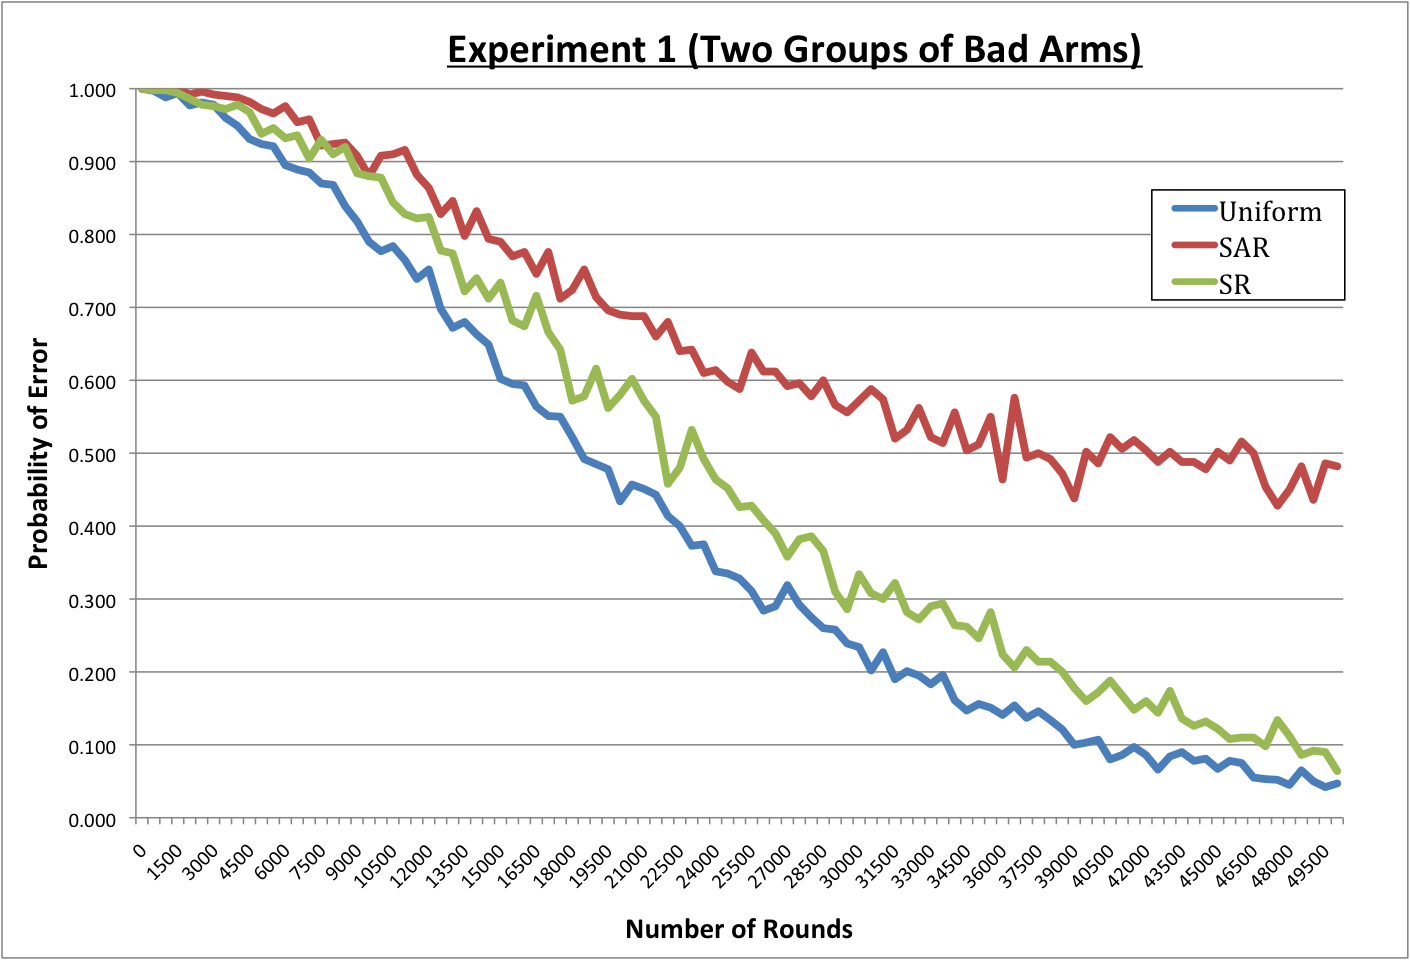
\includegraphics[width=75mm]{Experiment1.png}
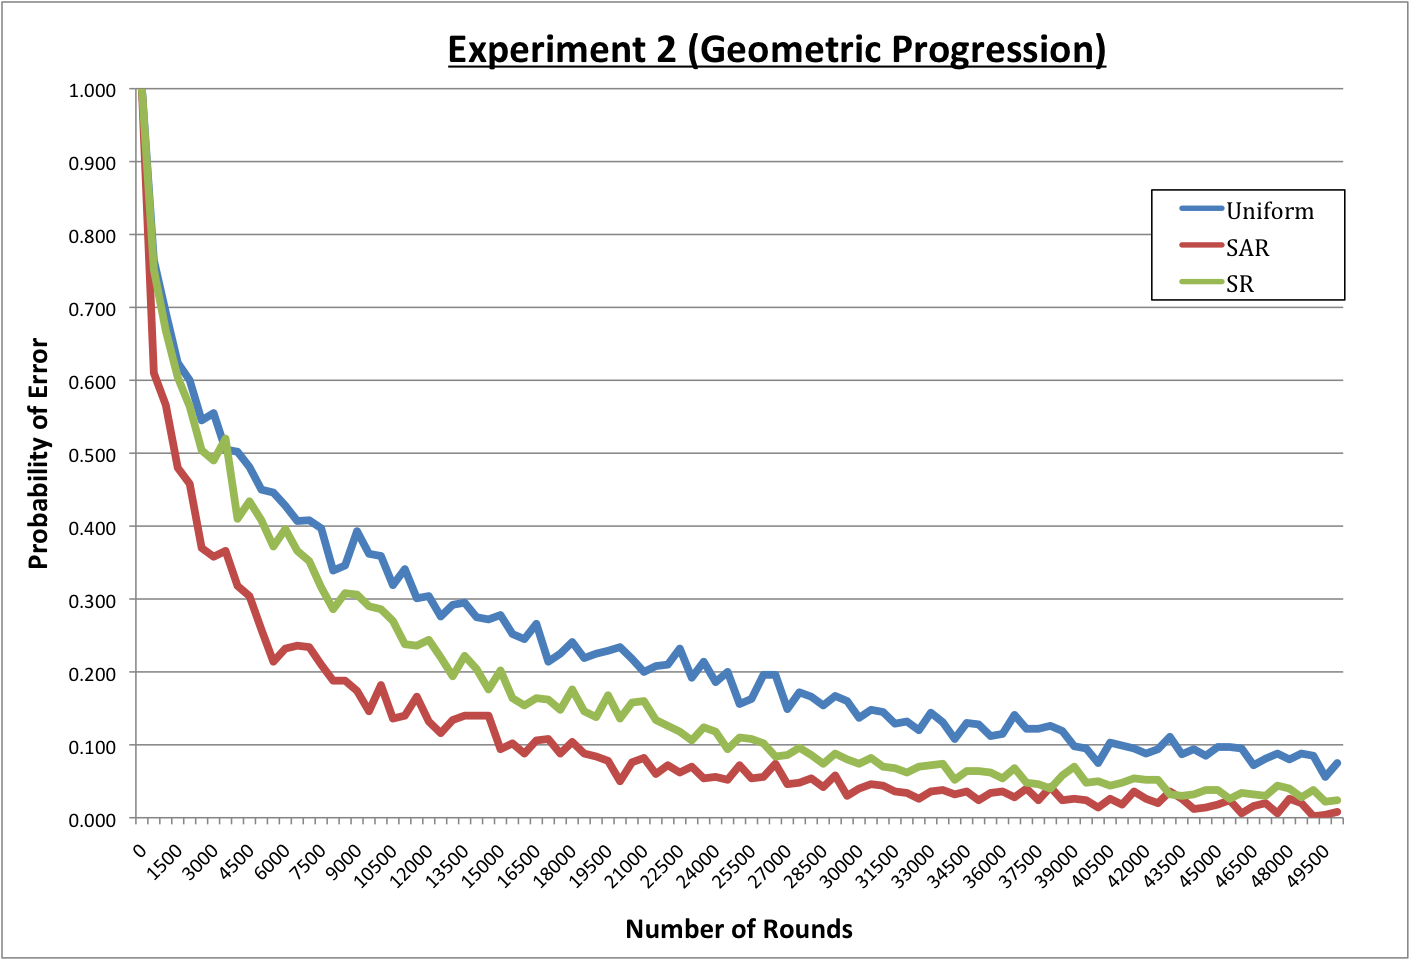
\includegraphics[width=75mm]{Experiment2.png}
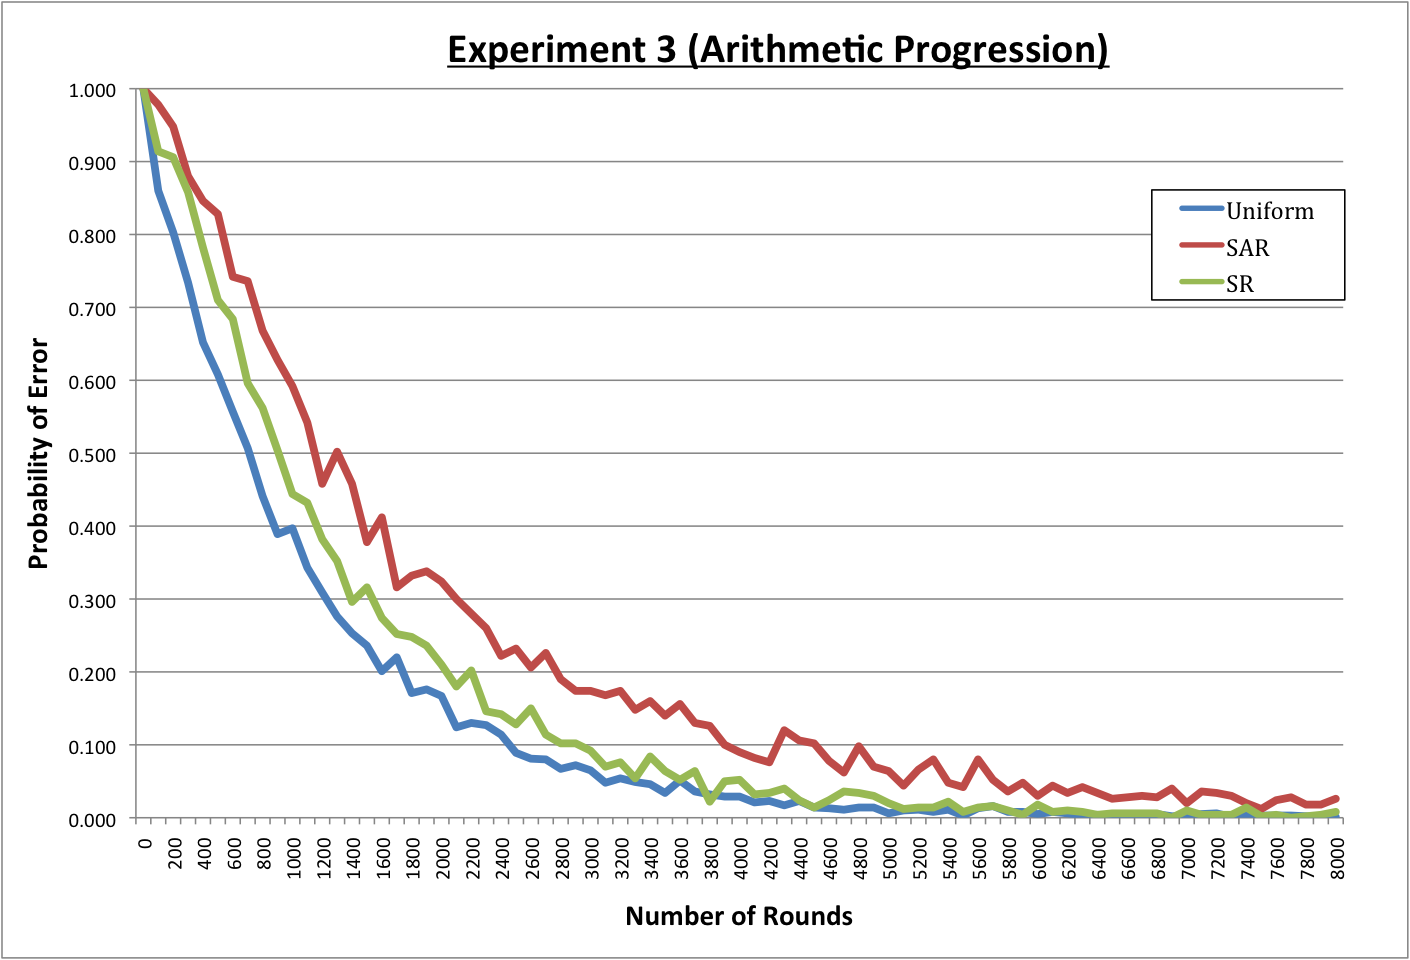
\includegraphics[width=75mm]{Experiment3.png}
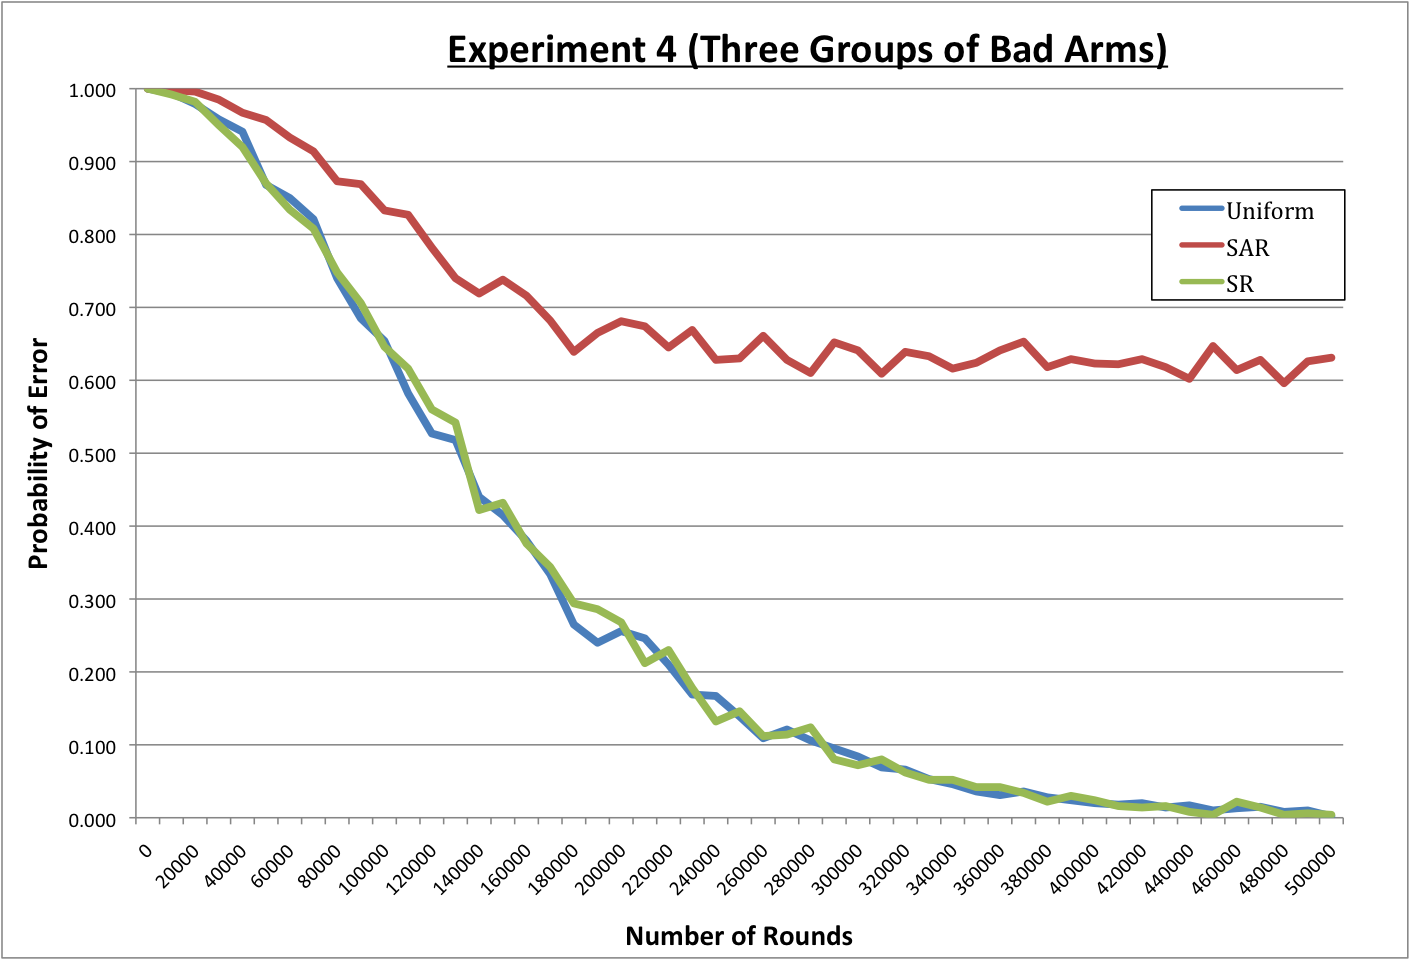
\includegraphics[width=75mm]{Experiment4.png}
\caption{\label{experiments} Simulation Results for Maximum Weighted Spanning Tree}
\end{figure}

Looking at the results in Fig. \ref{experiments} we see that our algorithms performed much worse than expected. On the whole Combinatorial SAR performs the worst between the two, however it does perform the best for Experiment 2. Additionally as we suggested, SAR struggles in scenarios where it has many bad arms to differentiate amongst, most notably in Experiment 4.\\

On the other hand, Combinatorial SR performs much better than SAR. Our strategy to not explicitly accept or reject arms seems to have worked as SR performs well in the two experiments with groups of bad arms. Ultimately though, it at beast does as well as Uniform but never better.\\

\section{Conclusion} \label{sec:con}
In this thesis we have studied combinatorial identification in multi-armed bandits. Our goal has been to find a generalized sampling strategy for dynamically changing edge-weights on combinatorial structures, that performs better than uniform sampling. Specifically we proposed two algorithms, Combinatorial SAR \& SR, which were extensions of previous work in \cite{ABM10} and \cite{BWV13}. Given the sucess of the two algorithms in the settings of $best$ and $mbest$ identification, we suspected they might extend to the general combinatorial setting. Despite finding the converse to be true, we consider our analysis and experimental results to be useful indicators of research direction. This particular problem has yet to be solved in any of the specific combinatorial settings that we considered, thus an attempt to solve the problem in general is not a trivial matter.\\

Given our limited theoretical understanding, we propose that further experiments should be considered. We believe that a proposed algorithmic solution will arrive from attempting several variations of existing sampling strategies and working backwards to develop a theoretical understanding. We dismiss the claim that one cannot do better than uniform sampling as clearly one can improve one's recommendation by not wasting samples on suboptimal arms. Ultimatley though, based on our results we find that an entirely new algorithm must be formulated.\\

\newpage
\appendix

\section{} \label{sec:app}
In this Appendix we prove several results stated earlier.

\subsection{Hoeffding's Inequality}
We use a simply stated version of Hoeffding's Inequality.

\begin{thm} Let $X_1, \hdots, X_n$ be independent identically distributed random variables with mean $\mu$, and bounded in the range [0,1], then
$$ \P(|\hat{X}_n - \mu| \ge t) \le 2e^{-2nt^2} = 2 \exp (-2nt^2)

\end{thm}

For proofs and other statements of Hoeffding's inequality see \cite{SINAI}.

\subsection{Kruskal's Algorithm}
We provide a simpler proof of Kruskal's Algorithm than in \cite{DW01}.

\begin{defn}
Let T be a spanning tree of G, and let f $\in E(G) - E(T)$. A cycle C of G with $f \in E(C)$ such that $C \setminus f$ is a path of T is called a \textbf{fundamental cycle of f with respect to T}.
\end{defn}

Proof of Kruskal's Algorithm.

\begin{proof}
Let $e_1,\hdots,e_{m}$ be the edges generated by Kruskal's algorithm. Choose $i \in \{1,\hdots,m\}$ maximum such that there is a minimum weighted spanning tree (mst) containing all of $e_1,\hdots,e_{i-1}$. We claim that $i = n$. Suppose to the contrary that $i \neq n$. Let T be a mst containing $e_1,\hdots,e_{i-1}$. Then $e_i \not \in  E(T)$ from the maximality of $i$. Let $C$ be the fundamental cycle of $e_i$ with respect to T. Since the algorithm chose edge $e_i$, there is no cycle in $\{e_1,\hdots,e_i\}$, and so some edge $e$ of $C$ is not in $\{e_1,\hdots,e_i\}$. There is no cycle included in $\{e_1,\hdots,e_{i-1},e\}$ since all these edges belong to T. Furthermore since the algorithm chose $e_i$ rather than $e$, it follows that $w(e_i) \le w(e)$. But since $e$ is an edge of the fundamental cycle of $e_i$ with respect to T, we have that $w(e_i) \ge w(e)$, hence $w(e_i) = w(e)$. Now note that we can construct a spanning tree $T'$ with edge-set $(E(T)\setminus{e}) \cup \{e_i\}$ and since $w(e_i)=w(e)$ it follows that $T'$ is a mst. Hence $e_1,...,e_i \in E(T')$ which contradicts the maximality of i.
\end{proof}

\nocite{*}
\newpage
\bibliographystyle{plain}
\bibliography{newbib_thesis}
\end{document}